% Created 2018-04-13 Fri 16:14
% Intended LaTeX compiler: pdflatex
\documentclass[10pt, compress, aspectratio=169, xcolor={table,usenames,dvipsnames}]{beamer}

\mode<beamer>{\usetheme[numbering=fraction, progressbar=none, titleformat=smallcaps, sectionpage=none]{metropolis}}
\usepackage{sourcecodepro}
\usepackage{booktabs}
\usepackage{array}
\usepackage{listings}
\usepackage{graphicx}
\usepackage[english]{babel}
\usepackage[scale=2]{ccicons}
\usepackage{url}
\usepackage{relsize}
\usepackage{wasysym}
\usepackage{ragged2e}
\usepackage{textcomp}
\usepackage{pgfplots}
\usepgfplotslibrary{dateplot}
\definecolor{Base}{HTML}{191F26}
\definecolor{Accent}{HTML}{157FFF}
\setbeamercolor{alerted text}{fg=Accent}
\setbeamercolor{frametitle}{bg=Base}
\setbeamercolor{normal text}{bg=black!2,fg=Base}
\setsansfont[BoldFont={Source Sans Pro Semibold},Numbers={OldStyle}]{Source Sans Pro}
\lstdefinelanguage{Julia}%
{morekeywords={abstract,struct,break,case,catch,const,continue,do,else,elseif,%
end,export,false,for,function,immutable,mutable,using,import,importall,if,in,%
macro,module,quote,return,switch,true,try,catch,type,typealias,%
while,<:,+,-,::,*,/},%
sensitive=true,%
alsoother={$},%
morecomment=[l]\#,%
morecomment=[n]{\#=}{=\#},%
morestring=[s]{"}{"},%
morestring=[m]{'}{'},%
}[keywords,comments,strings]%
\lstset{ %
backgroundcolor={},
basicstyle=\ttfamily\footnotesize,
breakatwhitespace=true,
breaklines=true,
captionpos=n,
commentstyle=\color{Accent},
escapeinside={\%*}{*)},
extendedchars=true,
frame=n,
keywordstyle=\color{Accent},
language=R,
rulecolor=\color{black},
showspaces=false,
showstringspaces=false,
showtabs=false,
stepnumber=2,
stringstyle=\color{gray},
tabsize=2,
}
\renewcommand*{\UrlFont}{\ttfamily\smaller\relax}
\graphicspath{{../img/}}
\addtobeamertemplate{block begin}{}{\justifying}
\usetheme{default}
\author{Pedro Bruel}
\date{\today}
\title{Autotuning: A Design of Experiments Approach}
\hypersetup{
 pdfauthor={Pedro Bruel},
 pdftitle={Autotuning: A Design of Experiments Approach},
 pdfkeywords={},
 pdfsubject={},
 pdfcreator={Emacs 25.3.1 (Org mode 9.1.9)}, 
 pdflang={English}}
\begin{document}

\maketitle
\begin{frame}{Outline}
\tableofcontents
\end{frame}


\section{Autotuning}
\label{sec:org6c0e495}
\begin{frame}[fragile,label={sec:orge1cf4d7}]{Autotuning: Optimizing Program Configurations}
 \begin{columns}
\begin{column}{0.5\columnwidth}
\begin{block}{Architectures for High Performance Computing}
\begin{center}

\includegraphics[width=.9\linewidth]{../img/architectures.png}
\end{center}

How to write \alert{efficient code} for each of these?

\begin{block}{Autotuning}
\vspace{.2cm}

The process of \alert{automatically finding} a \alert{configuration} of a program that
optimizes an \alert{objective}
\end{block}
\end{block}
\end{column}

\begin{column}{0.5\columnwidth}
\begin{block}{Configurations}
\begin{itemize}
\item Program Configuration
\begin{itemize}
\item Algorithm, block size, \(\dots\)
\end{itemize}
\item Source code transformation
\begin{itemize}
\item Loop unrolling, tiling, rotation \(\dots\)
\end{itemize}
\item Compiler configuration
\begin{itemize}
\item \texttt{-O2}, vectorization, \(\dots\)
\end{itemize}
\item \(\dots\)
\end{itemize}

\begin{block}{Objectives}
\begin{itemize}
\item Execution time
\item Memory \& power consumption
\item \(\dots\)
\end{itemize}
\end{block}
\end{block}
\end{column}
\end{columns}
\end{frame}

\begin{frame}[label={sec:org7cffd57}]{Autotuning: Search Spaces}
\begin{columns}
\begin{column}{0.5\columnwidth}
\begin{block}{Search Spaces}
\vspace{.2cm}

Represent the \alert{effect} of all possible
\alert{configurations} on the \alert{objectives}

Can be difficult to explore, with multiple \alert{local optima}
and \alert{undefined regions}
\end{block}
\end{column}

\begin{column}{0.5\columnwidth}
\begin{center}
\begin{center}
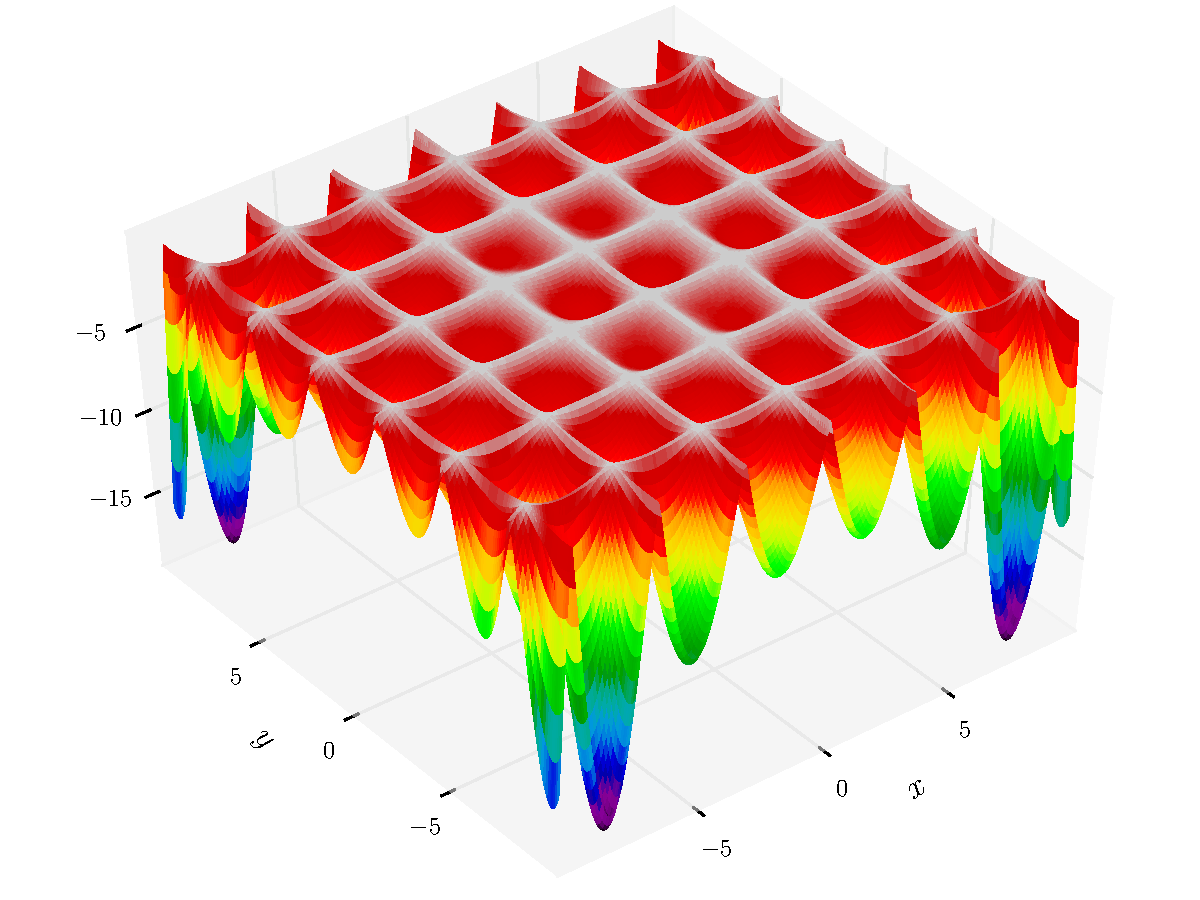
\includegraphics[width=.9\linewidth]{../img/holder_table.pdf}
\end{center}    

\alert{Hölder Table Function}
\end{center}
\end{column}
\end{columns}
\end{frame}

\begin{frame}[label={sec:org17a6269}]{Autotuning: Exploring Search Spaces}
\begin{columns}
\begin{column}{0.5\columnwidth}
\begin{block}{Issue 1: \alert{Exponential Growth}}
\vspace{.2cm}

\alert{Simple factors} can generate \alert{large spaces}:

\begin{itemize}
\item 30 \alert{boolean} factors
\item \(2^{30}\) combinations
\end{itemize}

\begin{block}{Issue 2: \alert{Geometry}}
\begin{itemize}
\item \alert{Discrete} or \alert{continous} factors
\item \alert{``Smoothness''}
\item \alert{Interactions} between factors
\end{itemize}
\end{block}
\end{block}
\end{column}

\begin{column}{0.5\columnwidth}
\begin{block}{Issue 3: \alert{Measurement Time}}
\vspace{.2cm}

Time to \alert{compile}:

\begin{itemize}
\item \alert{Benchmark} GPU applications: \alert{1\textasciitilde{}10s}
\item \alert{Benchmark} FPGA applications: \alert{1\textasciitilde{}10min}
\item \alert{Industrial} FPGA applications: \alert{1\textasciitilde{}10h}
\end{itemize}
\end{block}
\end{column}
\end{columns}
\end{frame}
\end{document}
